% Electronic supplementary material for the AAS manuscript. Compile with pdfLaTeX (separate document).
% v8 (2026-09-26): naming aligned with the main text (PS-PaE-Fuse; objective experiment), implementation
% notes of the objective experiment moved here from the main text, and Tables S10--S11 added.
\documentclass[12pt]{article}
\usepackage{atmosphere}
\newenvironment{Exercises}[1][10.]{
\refbt{REFERENCES}
\begin{list}
{\hfill }{
\settowidth{\labelwidth}{\bfseries #1}%
\setlength{\labelsep}{0pt}%
\setlength{\topsep}{0bp}%
\setlength{\partopsep}{0pt}%
\setlength{\parskip}{0pt}%
\setlength{\itemsep}{0bp}%
\setlength{\leftmargin}{\labelwidth+\labelsep}%
\usecounter{enumi}}}{\end{list}\smallskip}

\def\tablename{\bf Table}
\def\figurename{\bf Fig.~}

\newcommand{\refbt}[1]{\centering #1}

\def\acknowledgmentsname{{\it Acknowledgements}.\ }

\newcommand{\add}[1]{\vspace*{-19mm}\begin{center}{\small\it #1}\end{center}}

\newcommand{\keywords}[1]{
\begin{center}
\parbox[t]{153mm}{\noindent{\bf Keywords:}\ #1}
\end{center}}

\newcommand{\abs}[1]{\vspace*{-5mm}
\begin{center}
{\bf ABSTRACT}
\end{center}
\vspace*{-5mm}

#1}

\newcommand{\bte}[1]{\vspace*{3mm}\noindent #1}


\setlength{\parskip}{0mm}
\setlength{\arraycolsep}{0.5mm}

\makeatletter
\newskip\@footindent
\@footindent=2.5mm

\renewcommand\footnoterule{\kern6\p@ \hrule width 0.4\columnwidth \kern4\p@}
\@addtoreset{footnote}{page}

\renewcommand\thesection{\arabic{section}.}
\renewcommand\thesubsection{\arabic{section}.\arabic{subsection}}
\renewcommand\thesubsubsection{\arabic{section}.\arabic{subsection}.\arabic{subsubsection}}

\titleformat{\section}{\bf\normalsize}{\thesection}{.5em}{}
\titlespacing{\section}{0mm}{5mm}{0mm}

\titleformat{\subsection}{\bf\normalsize\it}{\thesubsection}{1em}{}
\titlespacing{\subsection}{0mm}{3mm}{0mm}

\titleformat{\subsubsection}{\normalfont\normalsize\it}{\thesubsubsection}{1em}{}
\titlespacing{\subsubsection}{0mm}{3mm}{0mm}

\titleformat{\paragraph}{\normalfont\normalsize\it}{\thesubsubsection}{1em}{}
\titlespacing{\subsubsection}{0mm}{3mm}{0mm}



\linespread{2} 
\usepackage{soul}
\usepackage{xurl}
\newcommand{\fitTable}[1]{\begingroup\linespread{1}\selectfont\setbox0=\hbox{#1}\ifdim\wd0>\linewidth\setbox0=\hbox{\resizebox{\linewidth}{!}{\box0}}\fi\ifdim\dimexpr\ht0+\dp0\relax>.68\textheight\resizebox*{!}{.68\textheight}{\box0}\else\box0\fi\endgroup}
\sethlcolor{yellow}
\newcommand{\todo}[1]{\hl{#1}}
\newcommand{\todobox}[1]{\par\noindent\colorbox{yellow}{\parbox{\dimexpr\linewidth-2\fboxsep\relax}{\small #1}}\par}
\newcommand{\mps}{m s$^{-1}$}
\graphicspath{{figures/}}
\renewcommand{\thetable}{S\arabic{table}}
\renewcommand{\thefigure}{S\arabic{figure}}

\begin{document}

\title{\vspace*{-20mm}\fontsize{12}{12}\bf
Electronic Supplementary Material for\\
Extreme-Aware Fusion of Multi-Model AI Weather Forecasts: Joint Optimization of Overall Skill and Event Detection
\vspace*{-3mm}}
\date{}
\author{\\[-17mm]\fontsize{12}{12}\colorbox{yellow}{Author list as in the main text}}
\maketitle

\noindent This file contains the implementation details of the linear-stacking objective experiment, Tables S1--S11 and Figs.~S1--S3 referred to in the main text. Values are reported from the archived evaluation records. The original table-generation scripts were not included in the supplied Overleaf archive.

\section{Implementation of the linear-stacking objective experiment}

The objective experiment isolates the training objective in the simplest model that can express a trade-off. A linear stacking with 90 parameters maps the four members to a fused field for each variable and lead time. For each of six variables and three lead times, four coefficients and one bias define a correction from the normalized member forecasts; the correction is multiplied by the training-only error scale and added to the arithmetic member mean, giving $(4+1)\times6\times3=90$ trainable coefficients. The training loss is
\begin{equation}
L_{\lambda} = \mathrm{nMSE} + \lambda\,\bigl(1 - \mathrm{CSI}^{\mathrm{soft}}_{20}\bigr),
\label{eq:jointS}
\end{equation}
where nMSE is the latitude-weighted mean-square error divided by the squared training-only RMSE of the arithmetic member mean for each variable and averaged over the six variables and three lead times. The event term uses $p=\mathrm{sigmoid}[(\sqrt{\hat u^2+\hat v^2+10^{-8}}-20)/\tau]$, with $\tau=1$ \mps\ and the observed indicator $o=\mathbb{1}(\sqrt{u^2+v^2}\geq20)$. Within each lead-time group, $\mathrm{CSI}^{\mathrm{soft}}_{20}=\sum wp o/[\sum w(p+o-po)+10^{-6}]$, where $w$ is the cosine-latitude weight; the event loss is averaged over the lead groups present in the batch. Four weights were trained: $\lambda = 0$ (overall error only), $\lambda = 0.15$, a tenfold $\lambda = 1.5$ and $\lambda = 3.18$ (unrounded: 3.181574748), obtained from the median initial gradient-norm ratio over 32 fixed training batches. Every model starts from the same ridge-regression initialization and uses AdamW for 16 epochs (batch size 24, learning rate $3\times10^{-4}$, weight decay $10^{-4}$), with three shuffle seeds (123, 456 and 789). The checkpoint is selected on the 2020 selection dates by minimizing the common functional $Q = \mathrm{nMSE} + 0.15\,(1 - \mathrm{CSI}_{20})$ evaluated on the safeguarded output, so that the $\lambda = 0$ control shares the selection rule and differs only in the training gradient. A 28-date diagnostic set of 2020 reports development behaviour (Table~\ref{tab:dev}). The 12 checkpoints were then frozen and evaluated on the 2021 sample without any further choice.

Every checkpoint is evaluated on its raw output and after a common wind-vector safeguard: where at least two members forecast wind speed of 15 \mps\ or more and the fastest member exceeds the fused speed, the fused U10 and V10 are blended toward the strongest member with weight $\alpha = 0.75$; the other four variables are untouched. The same rule is applied to the ridge initialization and to the simple mean, so that every comparison of a joint model has a matched control at both output stages. This rule differs from the PS-PaE-Fuse safeguard (local q95 trigger, $\alpha = 1$) in trigger and blending weight, so the objective experiment and PS-PaE-Fuse are separate experiments rather than one ablation ladder.

\clearpage
\section{Development-set behaviour of the joint objective (2020)}

Table~\ref{tab:dev} lists the 2020 selection-set and diagnostic-set scores of the four objectives of the linear-stacking experiment. The selection set was used to choose the checkpoint with the common functional $Q$; the diagnostic set was held out from that choice but belongs to the 2020 development cycle and is not an independent year. Both sets show the ordering that the frozen 2021 test reproduces at smaller amplitude.

\begin{table}[h!]
\caption{Development scores of the linear-stacking objective experiment on the 2020 selection set (36 dates) and diagnostic set (28 dates), three-seed means with the sample standard deviation over seeds in parentheses for CSI$_{20}$.}
\label{tab:dev}
\vspace*{2mm}
\centering
{\linespread{1.0}\selectfont\small
\fitTable{\begin{tabular}{llcccc}
\hline
Objective & Output & Selection nMSE & Selection CSI$_{20}$ & Diagnostic nMSE & Diagnostic CSI$_{20}$ \\
\hline
Overall error only, $\lambda=0$ & Raw & 0.8768 & 0.0401 (0.0006) & 0.8343 & 0.1059 (0.0009) \\
Overall error only, $\lambda=0$ & Safeguarded & 0.8791 & 0.1243 (0.0006) & 0.8365 & 0.2360 (0.0006) \\
Joint, $\lambda=0.15$ & Raw & 0.8769 & 0.0542 (0.0001) & 0.8341 & 0.1203 (0.0009) \\
Joint, $\lambda=0.15$ & Safeguarded & 0.8792 & 0.1294 (0.0000) & 0.8363 & 0.2384 (0.0002) \\
Joint, $\lambda=1.5$ & Raw & 0.8773 & 0.0703 (0.0065) & 0.8342 & 0.1429 (0.0018) \\
Joint, $\lambda=1.5$ & Safeguarded & 0.8797 & 0.1335 (0.0019) & 0.8364 & 0.2426 (0.0001) \\
Joint, gradient-calibrated $\lambda=3.18$ & Raw & 0.8774 & 0.0719 (0.0051) & 0.8342 & 0.1460 (0.0028) \\
Joint, gradient-calibrated $\lambda=3.18$ & Safeguarded & 0.8798 & 0.1348 (0.0019) & 0.8364 & 0.2441 (0.0002) \\
\hline
\end{tabular}
}}
\end{table}

\clearpage
\section{Six-variable results on the 2021 sample}

Table~\ref{tab:sixvar} gives the equal-lead RMSE of all six variables for the learned experts of PS-PaE-Fuse (before the safeguard) and the simple statistical controls on the coordinate-verified 2021 sample. Table~\ref{tab:sixcost} gives the per-variable, per-lead RMSE cost of the three joint objectives of the linear-stacking experiment relative to the $\lambda=0$ control at both output stages.

\begin{table}[h!]
\caption{Equal-lead RMSE over the 22 initialization dates of 2021 for the four members, four simple combinations, the global-skill expert and PS-PaE-Fuse without the safeguard for the three frozen router seeds. Z500 is geopotential in m$^{2}$ s$^{-2}$. Upper-air values use the coordinate-verified ERA5 reference.}
\label{tab:sixvar}
\vspace*{2mm}
\centering
{\linespread{1.0}\selectfont\footnotesize
\fitTable{\begin{tabular}{lcccccc}
\hline
System & T2M (K) & U10 (m s$^{-1}$) & V10 (m s$^{-1}$) & MSL (Pa) & Z500 (m$^2$ s$^{-2}$) & T850 (K) \\
\hline
Pangu-Weather & 1.5350 & 2.4576 & 2.5361 & 305.83 & 300.37 & 1.7955 \\
GraphCast & 1.4344 & 2.2617 & 2.3487 & 285.18 & 278.60 & 1.6568 \\
FuXi & 1.4559 & 2.1913 & 2.2934 & 277.72 & 271.34 & 1.6457 \\
ECMWF HRES & 1.8023 & 2.7448 & 2.8208 & 324.04 & 315.13 & 1.9615 \\
Simple mean & 1.2879 & 2.0551 & 2.1365 & 249.98 & 244.16 & 1.5014 \\
Mean-bias-corrected mean & 1.2918 & 2.0563 & 2.1366 & 250.07 & 243.71 & 1.5008 \\
Affine-calibrated mean & 1.2940 & 2.0546 & 2.1348 & 249.95 & 243.87 & 1.5004 \\
Disagreement-conditioned bias-corrected mean & 1.2995 & 2.0565 & 2.1374 & 250.24 & 243.69 & 1.5013 \\
Global-skill expert & 1.2799 & 2.0430 & 2.1447 & 253.40 & 247.38 & 1.5108 \\
PS-PaE-Fuse w/o safeguard, seed 123 & 1.2819 & 2.0432 & 2.1479 & 253.43 & 247.33 & 1.5157 \\
PS-PaE-Fuse w/o safeguard, seed 456 & 1.2781 & 2.0436 & 2.1493 & 253.37 & 247.29 & 1.5135 \\
PS-PaE-Fuse w/o safeguard, seed 789 & 1.2834 & 2.0434 & 2.1495 & 253.39 & 247.33 & 1.5171 \\
\hline
\end{tabular}
}}
\end{table}

\begin{table}[h!]
\caption{RMSE of the $\lambda=0$ control of the linear-stacking experiment by variable and lead time (three-seed means), and the relative RMSE change (\%) of the three joint objectives at the same output stage; negative values are lower error. The safeguard changes U10 and V10 only.}
\label{tab:sixcost}
\vspace*{2mm}
\centering
{\linespread{1.0}\selectfont\footnotesize
\fitTable{\begin{tabular}{llcccccc}
\hline
Variable & Unit & Lead (h) & Output & RMSE, $\lambda=0$ & $\Delta$RMSE (\%), $\lambda=0.15$ & $\lambda=1.5$ & $\lambda=3.18$ \\
\hline
T2M & K & 72 & Raw & 0.9045 & -0.006596 & -0.012349 & -0.012303 \\
U10 & m s$^{-1}$ & 72 & Raw & 1.3544 & +0.089182 & +0.313570 & +0.338227 \\
V10 & m s$^{-1}$ & 72 & Raw & 1.3932 & -0.021652 & +0.042451 & +0.057600 \\
MSL & Pa & 72 & Raw & 115.41 & +0.000333 & +0.002534 & +0.016267 \\
Z500 & m$^2$ s$^{-2}$ & 72 & Raw & 104.72 & -0.003036 & -0.010532 & -0.008493 \\
T850 & K & 72 & Raw & 0.9679 & +0.001414 & +0.000962 & +0.003917 \\
T2M & K & 120 & Raw & 1.2516 & +0.017011 & +0.006841 & +0.006830 \\
U10 & m s$^{-1}$ & 120 & Raw & 2.0591 & -0.000792 & +0.107096 & +0.130094 \\
V10 & m s$^{-1}$ & 120 & Raw & 2.1351 & -0.014728 & +0.026058 & +0.055942 \\
MSL & Pa & 120 & Raw & 245.57 & -0.033815 & -0.004524 & -0.000007 \\
Z500 & m$^2$ s$^{-2}$ & 120 & Raw & 233.44 & -0.008586 & -0.013231 & -0.005716 \\
T850 & K & 120 & Raw & 1.4624 & +0.000164 & -0.000908 & -0.001012 \\
T2M & K & 168 & Raw & 1.6623 & +0.016384 & +0.004651 & +0.004645 \\
U10 & m s$^{-1}$ & 168 & Raw & 2.6762 & -0.000378 & +0.002069 & +0.011559 \\
V10 & m s$^{-1}$ & 168 & Raw & 2.8284 & -0.006589 & -0.009527 & -0.006890 \\
MSL & Pa & 168 & Raw & 385.32 & -0.021794 & +0.012939 & +0.012655 \\
Z500 & m$^2$ s$^{-2}$ & 168 & Raw & 387.71 & -0.004722 & -0.004639 & -0.004518 \\
T850 & K & 168 & Raw & 2.0338 & -0.006569 & +0.000890 & -0.000354 \\
T2M & K & 72 & Safeguarded & 0.9045 & -0.006596 & -0.012349 & -0.012303 \\
U10 & m s$^{-1}$ & 72 & Safeguarded & 1.3662 & +0.098835 & +0.317257 & +0.340733 \\
V10 & m s$^{-1}$ & 72 & Safeguarded & 1.4059 & -0.009364 & +0.053565 & +0.068389 \\
MSL & Pa & 72 & Safeguarded & 115.41 & +0.000333 & +0.002534 & +0.016267 \\
Z500 & m$^2$ s$^{-2}$ & 72 & Safeguarded & 104.72 & -0.003036 & -0.010532 & -0.008493 \\
T850 & K & 72 & Safeguarded & 0.9679 & +0.001414 & +0.000962 & +0.003917 \\
T2M & K & 120 & Safeguarded & 1.2516 & +0.017011 & +0.006841 & +0.006830 \\
U10 & m s$^{-1}$ & 120 & Safeguarded & 2.0817 & +0.011327 & +0.124704 & +0.147315 \\
V10 & m s$^{-1}$ & 120 & Safeguarded & 2.1587 & -0.010813 & +0.032427 & +0.061269 \\
MSL & Pa & 120 & Safeguarded & 245.57 & -0.033815 & -0.004524 & -0.000007 \\
Z500 & m$^2$ s$^{-2}$ & 120 & Safeguarded & 233.44 & -0.008586 & -0.013231 & -0.005716 \\
T850 & K & 120 & Safeguarded & 1.4624 & +0.000164 & -0.000908 & -0.001012 \\
T2M & K & 168 & Safeguarded & 1.6623 & +0.016384 & +0.004651 & +0.004645 \\
U10 & m s$^{-1}$ & 168 & Safeguarded & 2.7009 & +0.000610 & +0.006645 & +0.019865 \\
V10 & m s$^{-1}$ & 168 & Safeguarded & 2.8505 & -0.004367 & -0.004203 & +0.000060 \\
MSL & Pa & 168 & Safeguarded & 385.32 & -0.021794 & +0.012939 & +0.012655 \\
Z500 & m$^2$ s$^{-2}$ & 168 & Safeguarded & 387.71 & -0.004722 & -0.004639 & -0.004518 \\
T850 & K & 168 & Safeguarded & 2.0338 & -0.006569 & +0.000890 & -0.000354 \\
\hline
\end{tabular}
}}
\end{table}

\clearpage
\section{Weather-type stratification: full paired table}

\begin{table}[h!]
\linespread{1}\selectfont
\caption{All paired comparisons of the weather-type stratification on the sealed 2022 sample (seed 123), with 95\% intervals from 2\,000 resamples of the stratum units. Tropical cyclones: 92 storm identifiers (81 with an event); cold surge and non-tropical high wind: 32 initialization dates. U10 RMSE and CRPS are computed on observed event cells; Brier scores are available only for the probabilistic outputs of PS-PaE-Fuse.}
\label{tab:wt}
\vspace*{2mm}
\centering
{\linespread{1.0}\selectfont\footnotesize
\fitTable{\begin{tabular}{llcccc}
\hline
Stratum & Metric & Baseline & PS-PaE-Fuse & Difference & 95\% CI \\
\hline
\multicolumn{6}{l}{\textit{PS-PaE-Fuse minus Pangu-Weather}} \\
Tropical cyclone & U10 RMSE & 4.446 & 4.603 & +0.157 & [-0.181, +0.522] \\
Tropical cyclone & CSI & 0.453 & 0.495 & +0.042 & [+0.017, +0.067] \\
Tropical cyclone & POD & 0.537 & 0.587 & +0.050 & [+0.016, +0.083] \\
Tropical cyclone & FAR & 0.256 & 0.240 & -0.017 & [-0.041, +0.004] \\
Tropical cyclone & FSS9 & 0.767 & 0.803 & +0.036 & [+0.012, +0.065] \\
Cold surge & U10 RMSE & 2.759 & 2.207 & -0.551 & [-0.725, -0.406] \\
Cold surge & CSI & 0.386 & 0.439 & +0.053 & [+0.023, +0.093] \\
Cold surge & POD & 0.548 & 0.668 & +0.120 & [+0.067, +0.187] \\
Cold surge & FAR & 0.435 & 0.439 & +0.004 & [-0.051, +0.030] \\
Cold surge & FSS9 & 0.715 & 0.764 & +0.050 & [+0.011, +0.121] \\
Non-TC high wind & U10 RMSE & 6.302 & 5.937 & -0.365 & [-0.665, -0.072] \\
Non-TC high wind & CSI & 0.210 & 0.245 & +0.036 & [+0.019, +0.053] \\
Non-TC high wind & POD & 0.284 & 0.443 & +0.159 & [+0.130, +0.187] \\
Non-TC high wind & FAR & 0.556 & 0.645 & +0.089 & [+0.059, +0.120] \\
Non-TC high wind & FSS9 & 0.477 & 0.554 & +0.077 & [+0.045, +0.110] \\
\multicolumn{6}{l}{\textit{PS-PaE-Fuse minus PS-PaE-Fuse w/o safeguard}} \\
Tropical cyclone & U10 RMSE & 4.056 & 4.603 & +0.548 & [+0.337, +0.792] \\
Tropical cyclone & U10 CRPS & 2.128 & 2.268 & +0.140 & [+0.079, +0.207] \\
Tropical cyclone & CSI & 0.324 & 0.495 & +0.172 & [+0.137, +0.206] \\
Tropical cyclone & POD & 0.336 & 0.587 & +0.251 & [+0.214, +0.288] \\
Tropical cyclone & FAR & 0.103 & 0.240 & +0.136 & [+0.114, +0.161] \\
Tropical cyclone & FSS9 & 0.599 & 0.803 & +0.204 & [+0.158, +0.254] \\
Tropical cyclone & Brier & 0.13739 & 0.12348 & -0.01391 & [-0.02147, -0.00681] \\
Cold surge & U10 RMSE & 2.128 & 2.207 & +0.080 & [+0.028, +0.150] \\
Cold surge & U10 CRPS & 1.040 & 1.067 & +0.027 & [+0.014, +0.043] \\
Cold surge & CSI & 0.404 & 0.439 & +0.035 & [-0.022, +0.121] \\
Cold surge & POD & 0.463 & 0.668 & +0.205 & [+0.142, +0.295] \\
Cold surge & FAR & 0.240 & 0.439 & +0.199 & [+0.147, +0.255] \\
Cold surge & FSS9 & 0.719 & 0.764 & +0.045 & [-0.018, +0.197] \\
Cold surge & Brier & 0.02974 & 0.03278 & +0.00304 & [+0.00126, +0.00525] \\
Non-TC high wind & U10 RMSE & 5.907 & 5.937 & +0.029 & [-0.210, +0.305] \\
Non-TC high wind & U10 CRPS & 3.207 & 3.151 & -0.056 & [-0.153, +0.053] \\
Non-TC high wind & CSI & 0.170 & 0.245 & +0.076 & [+0.051, +0.107] \\
Non-TC high wind & POD & 0.179 & 0.443 & +0.264 & [+0.223, +0.306] \\
Non-TC high wind & FAR & 0.235 & 0.645 & +0.410 & [+0.362, +0.463] \\
Non-TC high wind & FSS9 & 0.400 & 0.554 & +0.153 & [+0.105, +0.214] \\
Non-TC high wind & Brier & 0.00091 & 0.00156 & +0.00065 & [+0.00059, +0.00073] \\
\hline
\end{tabular}
}}
\end{table}

\clearpage
\section{Seasonal values of the 2022 scorecard}

\begin{table}[h!]
\caption{Numerical values plotted in Fig.~2 of the main text: equal-lead scores over all 32 sealed 2022 dates and by season (7, 8, 8 and 9 dates in DJF, MAM, JJA and SON). PS-PaE-Fuse rows are three-seed means.}
\label{tab:seasonal}
\vspace*{2mm}
\centering
{\linespread{1.0}\selectfont\footnotesize
\fitTable{\begin{tabular}{llccccc}
\hline
Metric & System & All 32 & DJF & MAM & JJA & SON \\
\hline
U10 RMSE (m s$^{-1}$) & Pangu-Weather & 2.530 & 2.450 & 2.595 & 2.526 & 2.535 \\
 & GraphCast & 2.386 & 2.302 & 2.472 & 2.421 & 2.341 \\
 & FuXi & 2.290 & 2.294 & 2.353 & 2.250 & 2.264 \\
 & ECMWF HRES & 2.797 & 2.734 & 2.859 & 2.750 & 2.829 \\
 & Simple mean & 2.128 & 2.075 & 2.171 & 2.123 & 2.132 \\
 & EMOS & 2.124 & 2.074 & 2.175 & 2.120 & 2.117 \\
 & PS-PaE-Fuse w/o safeguard & 2.123 & 2.076 & 2.175 & 2.118 & 2.116 \\
 & PS-PaE-Fuse & 2.168 & 2.127 & 2.214 & 2.151 & 2.172 \\[5pt]
CSI, q97.5 & Pangu-Weather & 0.286 & 0.304 & 0.265 & 0.273 & 0.299 \\
 & GraphCast & 0.235 & 0.254 & 0.221 & 0.208 & 0.255 \\
 & FuXi & 0.263 & 0.259 & 0.237 & 0.263 & 0.285 \\
 & ECMWF HRES & 0.248 & 0.258 & 0.232 & 0.251 & 0.251 \\
 & Simple mean & 0.276 & 0.289 & 0.251 & 0.272 & 0.291 \\
 & EMOS & 0.224 & 0.230 & 0.200 & 0.215 & 0.245 \\
 & PS-PaE-Fuse w/o safeguard & 0.274 & 0.281 & 0.246 & 0.270 & 0.294 \\
 & PS-PaE-Fuse & 0.344 & 0.358 & 0.321 & 0.341 & 0.355 \\[5pt]
FSS$_9$, q97.5 & Pangu-Weather & 0.603 & 0.627 & 0.580 & 0.582 & 0.620 \\
 & GraphCast & 0.509 & 0.540 & 0.492 & 0.463 & 0.537 \\
 & FuXi & 0.541 & 0.529 & 0.501 & 0.549 & 0.570 \\
 & ECMWF HRES & 0.598 & 0.618 & 0.582 & 0.599 & 0.592 \\
 & Simple mean & 0.564 & 0.581 & 0.527 & 0.564 & 0.579 \\
 & EMOS & 0.466 & 0.471 & 0.424 & 0.458 & 0.497 \\
 & PS-PaE-Fuse w/o safeguard & 0.557 & 0.562 & 0.515 & 0.556 & 0.582 \\
 & PS-PaE-Fuse & 0.678 & 0.694 & 0.655 & 0.677 & 0.686 \\[5pt]
CSI, 20 m s$^{-1}$ & Pangu-Weather & 0.219 & 0.274 & 0.202 & 0.201 & 0.188 \\
 & GraphCast & 0.145 & 0.168 & 0.158 & 0.131 & 0.118 \\
 & FuXi & 0.162 & 0.173 & 0.137 & 0.160 & 0.160 \\
 & ECMWF HRES & 0.186 & 0.229 & 0.160 & 0.168 & 0.169 \\
 & Simple mean & 0.172 & 0.212 & 0.149 & 0.161 & 0.145 \\
 & EMOS & 0.128 & 0.134 & 0.113 & 0.126 & 0.122 \\
 & PS-PaE-Fuse w/o safeguard & 0.161 & 0.180 & 0.154 & 0.152 & 0.146 \\
 & PS-PaE-Fuse & 0.241 & 0.297 & 0.221 & 0.213 & 0.213 \\
\hline
\end{tabular}
}}
\end{table}

\clearpage
\section{Diagnostics of observed wind at or above 25 \mps}

\begin{table}[h!]
\caption{Area-weighted decomposition of the observed 2022 area with wind speed at or above 25 \mps\ (32 dates, three-seed means). ``No member reaches 25 \mps'' and ``fewer than two supporting members'' are not mutually exclusive categories. The mean shortfall is the fused forecast speed deficit averaged over missed cells.}
\label{tab:diag25}
\vspace*{2mm}
\centering
{\linespread{1.0}\selectfont\small
\fitTable{\begin{tabular}{lccc}
\hline
Quantity (area-weighted, three-seed mean) & 72 h & 120 h & 168 h \\
\hline
Missed by PS-PaE-Fuse w/o safeguard & 87.1\% & 89.1\% & 100.0\% \\
Missed by PS-PaE-Fuse & 45.2\% & 68.5\% & 91.4\% \\
No member reaches 25 m s$^{-1}$ & 45.2\% & 65.8\% & 90.2\% \\
Fewer than two supporting members & 4.2\% & 14.7\% & 66.3\% \\
Gate active on observed event cells & 95.4\% & 85.1\% & 33.7\% \\
Misses forecast at 20--25 m s$^{-1}$ & 75.9\% & 77.1\% & 16.1\% \\
Mean shortfall on misses (m s$^{-1}$) & 4.84 & 5.58 & 13.43 \\
\hline
\end{tabular}
}}
\end{table}

\clearpage
\section{Calendar-block sensitivity of the 2021 paired differences}

\begin{table}[h!]
\caption{CSI$_{20}$ differences between each joint objective of the linear-stacking experiment and the $\lambda=0$ control on the 2021 sample, with 95\% intervals from resampling initialization dates, 7-day calendar blocks and 14-day calendar blocks (2\,000 draws each). Intervals are pointwise sensitivity intervals of a sparse reused sample.}
\label{tab:calendar}
\vspace*{2mm}
\centering
{\linespread{1.0}\selectfont\small
\fitTable{\begin{tabular}{llccc}
\hline
Comparison & Output & Dates (22 units) & 7-day blocks (13 units) & 14-day blocks (7 units) \\
\hline
\shortstack[l]{Joint $\lambda=0.15$\\minus $\lambda=0$} & Raw & \shortstack{+0.0085\\{[+0.0056, +0.0111]}} & \shortstack{+0.0085\\{[+0.0052, +0.0111]}} & \shortstack{+0.0085\\{[+0.0055, +0.0102]}} \\
\shortstack[l]{Joint $\lambda=0.15$\\minus $\lambda=0$} & Safeguarded & \shortstack{-0.0005\\{[-0.0012, +0.0003]}} & \shortstack{-0.0005\\{[-0.0012, +0.0002]}} & \shortstack{-0.0005\\{[-0.0013, +0.0003]}} \\
\shortstack[l]{Joint $\lambda=1.5$\\minus $\lambda=0$} & Raw & \shortstack{+0.0160\\{[+0.0097, +0.0220]}} & \shortstack{+0.0160\\{[+0.0096, +0.0213]}} & \shortstack{+0.0160\\{[+0.0095, +0.0197]}} \\
\shortstack[l]{Joint $\lambda=1.5$\\minus $\lambda=0$} & Safeguarded & \shortstack{-0.0016\\{[-0.0031, +0.0000]}} & \shortstack{-0.0016\\{[-0.0031, -0.0001]}} & \shortstack{-0.0016\\{[-0.0032, -0.0001]}} \\
\shortstack[l]{Joint $\lambda=3.18$\\minus $\lambda=0$} & Raw & \shortstack{+0.0173\\{[+0.0106, +0.0237]}} & \shortstack{+0.0173\\{[+0.0105, +0.0231]}} & \shortstack{+0.0173\\{[+0.0102, +0.0215]}} \\
\shortstack[l]{Joint $\lambda=3.18$\\minus $\lambda=0$} & Safeguarded & \shortstack{-0.0016\\{[-0.0033, +0.0001]}} & \shortstack{-0.0016\\{[-0.0033, -0.0000]}} & \shortstack{-0.0016\\{[-0.0033, -0.0001]}} \\
\hline
\end{tabular}
}}
\end{table}

\clearpage
\section{Alert-frequency migration of the development-matched control}

\begin{table}[h!]
\caption{Alert-area fractions of the development-matched control: the target and achieved frequencies on the 2020 development fields, and the frequencies of the safeguarded simple mean and of the control on the 32 sealed 2022 dates. The 25 \mps\ cell at 120 h has a zero development target and is descriptive only.}
\label{tab:alertmig}
\vspace*{2mm}
\centering
{\linespread{1.0}\selectfont\small
\fitTable{\begin{tabular}{llcccc}
\hline
Lead (h) & Event & Dev. target (\%) & Dev. achieved (\%) & 2022 safeguard (\%) & 2022 matched control (\%) \\
\hline
72 & q95 & 4.338 & 4.338 & 4.702 & 5.055 \\
72 & q97.5 & 3.190 & 3.190 & 3.575 & 3.806 \\
72 & 15 & 1.460 & 1.460 & 1.832 & 1.913 \\
72 & 20 & 0.111 & 0.111 & 0.178 & 0.213 \\
72 & 25 & 0.002 & 0.002 & 0.013 & 0.019 \\
120 & q95 & 3.486 & 3.486 & 4.285 & 4.498 \\
120 & q97.5 & 2.574 & 2.574 & 3.350 & 3.558 \\
120 & 15 & 1.143 & 1.143 & 1.632 & 1.473 \\
120 & 20 & 0.074 & 0.074 & 0.183 & 0.139 \\
120 & 25 & 0.000 & 0.000 & 0.009 & 0.011 \\
168 & q95 & 2.620 & 2.620 & 3.082 & 3.079 \\
168 & q97.5 & 2.058 & 2.058 & 2.477 & 2.545 \\
168 & 15 & 0.832 & 0.832 & 0.821 & 0.805 \\
168 & 20 & 0.100 & 0.100 & 0.090 & 0.048 \\
168 & 25 & 0.001 & 0.001 & 0.005 & 0.008 \\
\hline
\end{tabular}
}}
\end{table}

\clearpage
\section{Development-set probabilistic calibration heads (candidate results)}

The main text reports that a single shared scale factor recovers about one third of the Brier-score loss caused by the safeguard. Two development-set experiments explored learned calibration heads on top of the fixed fused mean; both used reused 2020 dates and neither has been confirmed on external data, so they are candidates rather than results. Table~\ref{tab:heads} lists the headline scores as archived in the development result files.

\begin{table}[h!]
\linespread{1}\selectfont
\caption{Development-set scores of probabilistic calibration heads (2020 data only). ``Pilot'' rows: a 3\,303-parameter conditional head evaluated on a 10-date head hold-out; ``joint'' rows: the same head trained with and without a tail Brier term on a reused 8-date validation set. Normalized CRPS is averaged over the six variables. Values are archived development scores and are not comparable with the 2022 numbers of the main text.}
\label{tab:heads}
\vspace*{2mm}
\centering
{\linespread{1.0}\selectfont\small
\begin{tabular}{lcc}
\hline
Head & Mean normalized CRPS & Brier, q97.5 wind \\
\hline
Pilot: shared scale 1.6 & 0.2931 & 0.02549 \\
Pilot: common forecast features & 0.2898 & 0.02637 \\
Pilot: final-state features & 0.2906 & 0.02570 \\
Pilot: final-state and phase features & 0.2921 & 0.02648 \\
Joint: CRPS and U/V joint likelihood & 0.3010 & 0.02384 \\
Joint: with tail Brier term & 0.2967 & 0.02373 \\
\hline
\end{tabular}}
\end{table}
\noindent The pilot rows correspond to the archived keys \path{historical_1p6}, \path{common_only}, \path{final_state}, and \path{final_state_phase}; the joint rows correspond to \path{reference} and \path{A2}. Their displayed values have been checked against the archived development metrics. These experiments used historical cached verification fields and remain development-only diagnostics; they do not establish a result on the coordinate-corrected upper-air reference or an external year.

\clearpage
\section{Paired differences of the linear-stacking objective experiment (2021)}

\begin{table}[h!]
\caption{Paired differences of the linear-stacking objective experiment on the 2021 sample with 95\% intervals from 2\,000 draws of initialization dates (same draws for all systems, seed differences averaged within date). Positive $\Delta$CSI$_{20}$ favours the first-named system; negative $\Delta$nMSE and $\Delta Q$ favour it.}
\label{tab:paired}
\vspace*{2mm}
\centering
{\linespread{1.0}\selectfont\small
\fitTable{\begin{tabular}{llccc}
\hline
Comparison & Output & $\Delta$nMSE [95\% CI] & $\Delta$CSI$_{20}$ [95\% CI] & $\Delta Q$ [95\% CI] \\
\hline
\shortstack[l]{Joint $\lambda=0.15$\\minus $\lambda=0$} & Raw & \shortstack{-0.00005\\{[-0.00015, +0.00003]}} & \shortstack{+0.0085\\{[+0.0056, +0.0111]}} & \shortstack{-0.0013\\{[-0.0018, -0.0009]}} \\
\shortstack[l]{Joint $\lambda=0.15$\\minus $\lambda=0$} & Safeguarded & \shortstack{-0.00002\\{[-0.00011, +0.00005]}} & \shortstack{-0.0005\\{[-0.0012, +0.0003]}} & \shortstack{+0.0000\\{[-0.0001, +0.0002]}} \\
\shortstack[l]{Joint $\lambda=1.5$\\minus $\lambda=0$} & Raw & \shortstack{+0.00028\\{[+0.00008, +0.00046]}} & \shortstack{+0.0160\\{[+0.0097, +0.0220]}} & \shortstack{-0.0021\\{[-0.0031, -0.0011]}} \\
\shortstack[l]{Joint $\lambda=1.5$\\minus $\lambda=0$} & Safeguarded & \shortstack{+0.00033\\{[+0.00015, +0.00050]}} & \shortstack{-0.0016\\{[-0.0031, +0.0000]}} & \shortstack{+0.0006\\{[+0.0002, +0.0009]}} \\
\shortstack[l]{Joint $\lambda=3.18$\\minus $\lambda=0$} & Raw & \shortstack{+0.00037\\{[+0.00013, +0.00060]}} & \shortstack{+0.0173\\{[+0.0106, +0.0237]}} & \shortstack{-0.0022\\{[-0.0033, -0.0011]}} \\
\shortstack[l]{Joint $\lambda=3.18$\\minus $\lambda=0$} & Safeguarded & \shortstack{+0.00043\\{[+0.00021, +0.00064]}} & \shortstack{-0.0016\\{[-0.0033, +0.0001]}} & \shortstack{+0.0007\\{[+0.0003, +0.0010]}} \\[5pt]
\shortstack[l]{Joint $\lambda=0.15$\\minus Ridge} & Safeguarded & \shortstack{+0.00005\\{[-0.00002, +0.00013]}} & \shortstack{-0.0005\\{[-0.0013, +0.0003]}} & \shortstack{+0.0001\\{[-0.0000, +0.0003]}} \\
\shortstack[l]{Joint $\lambda=1.5$\\minus Ridge} & Safeguarded & \shortstack{+0.00041\\{[+0.00023, +0.00058]}} & \shortstack{-0.0016\\{[-0.0032, -0.0000]}} & \shortstack{+0.0007\\{[+0.0003, +0.0010]}} \\
\shortstack[l]{Joint $\lambda=3.18$\\minus Ridge} & Safeguarded & \shortstack{+0.00051\\{[+0.00030, +0.00072]}} & \shortstack{-0.0017\\{[-0.0033, +0.0000]}} & \shortstack{+0.0008\\{[+0.0004, +0.0011]}} \\
\shortstack[l]{Joint $\lambda=0.15$\\minus simple mean} & Safeguarded & \shortstack{-0.02094\\{[-0.02883, -0.01347]}} & \shortstack{-0.0011\\{[-0.0025, +0.0003]}} & \shortstack{-0.0208\\{[-0.0287, -0.0133]}} \\
\shortstack[l]{Joint $\lambda=1.5$\\minus simple mean} & Safeguarded & \shortstack{-0.02059\\{[-0.02842, -0.01317]}} & \shortstack{-0.0022\\{[-0.0034, -0.0011]}} & \shortstack{-0.0203\\{[-0.0282, -0.0128]}} \\
\shortstack[l]{Joint $\lambda=3.18$\\minus simple mean} & Safeguarded & \shortstack{-0.02048\\{[-0.02830, -0.01307]}} & \shortstack{-0.0023\\{[-0.0034, -0.0011]}} & \shortstack{-0.0201\\{[-0.0281, -0.0127]}} \\
\hline
\end{tabular}
}}
\end{table}

\clearpage
\section{Interaction of the joint objective with the common safeguard (2021)}

\begin{table}[h!]
\caption{Interaction of the joint objective with the common safeguard on the 2021 sample for 20 \mps\ events, by lead time (three-seed means). ``Own raw$\to$safeguarded'' is the CSI change produced by the safeguard on the joint model itself; the two ``Joint $-$ MSE'' columns are the differences to the $\lambda=0$ control before and after the safeguard; the hit and false-alarm terms are the symmetric algebraic decomposition of the safeguarded difference; $I$ is the equal-lead interaction (safeguarded difference minus raw difference) with its leave-one-date-out range.}
\label{tab:interaction}
\vspace*{2mm}
\centering
{\linespread{1.0}\selectfont\small
\fitTable{\begin{tabular}{lcccccc}
\hline
Objective & Lead (h) & \shortstack{Own raw$\to$guard\\$\Delta$CSI} & \shortstack{Joint $-$ MSE\\Raw} & \shortstack{Joint $-$ MSE\\Safeguarded} & Hit term & \shortstack{False-alarm\\term} \\
\hline
$\lambda=0.15$ & 72 & +0.0120 & +0.0102 & -0.0025 & +0.0044 & -0.0069 \\
 & 120 & +0.0963 & +0.0149 & +0.0005 & +0.0035 & -0.0030 \\
 & 168 & +0.0549 & +0.0003 & +0.0005 & +0.0006 & -0.0001 \\
 & \shortstack{Equal-lead\\interaction} & \multicolumn{5}{l}{$I = -0.0089$ [-0.0093, -0.0082]} \\[5pt]
$\lambda=1.5$ & 72 & +0.0058 & +0.0123 & -0.0065 & +0.0079 & -0.0144 \\
 & 120 & +0.0767 & +0.0348 & +0.0008 & +0.0089 & -0.0081 \\
 & 168 & +0.0549 & +0.0008 & +0.0010 & +0.0013 & -0.0003 \\
 & \shortstack{Equal-lead\\interaction} & \multicolumn{5}{l}{$I = -0.0176$ [-0.0184, -0.0160]} \\[5pt]
$\lambda=3.18$ & 72 & +0.0046 & +0.0129 & -0.0071 & +0.0083 & -0.0153 \\
 & 120 & +0.0738 & +0.0378 & +0.0009 & +0.0099 & -0.0089 \\
 & 168 & +0.0549 & +0.0011 & +0.0013 & +0.0018 & -0.0006 \\
 & \shortstack{Equal-lead\\interaction} & \multicolumn{5}{l}{$I = -0.0189$ [-0.0198, -0.0172]} \\
\hline
\end{tabular}
}}
\end{table}

\clearpage
\section{Per-lead detection scores of the linear-stacking objectives}

\begin{figure}[h!]
\centering
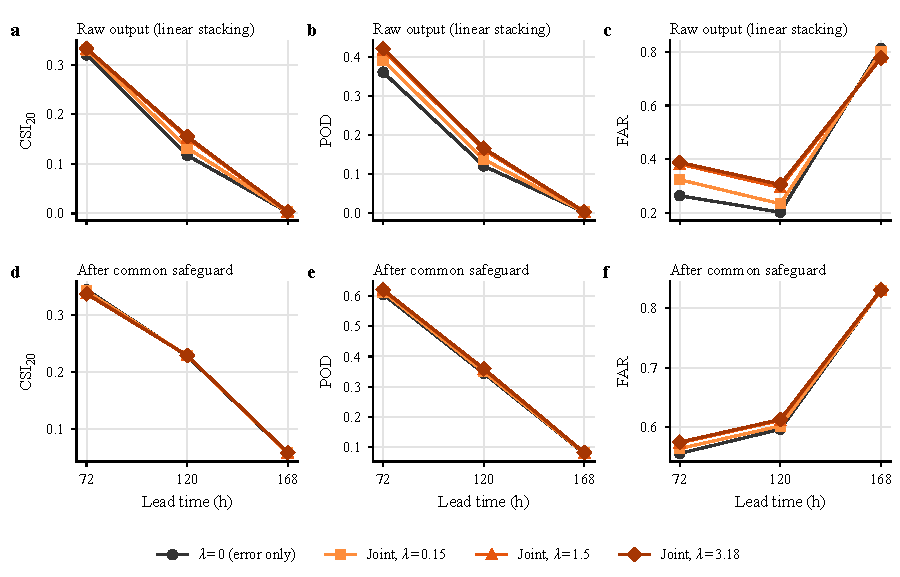
\includegraphics[width=\textwidth]{figS_lead_2021.pdf}
\caption{CSI, POD and FAR for 20 \mps\ wind events on the 2021 sample by lead time (three-seed means) for the four training objectives of the linear-stacking experiment, (a--c) on raw output and (d--f) after the common safeguard. At 168 h the 20 \mps\ CSI of every system is close to zero and the differences are not meaningful.}
\label{fig:lead}
\end{figure}


\clearpage
\section{Weather-type scores by lead time}

\begin{figure}[h!]
\centering
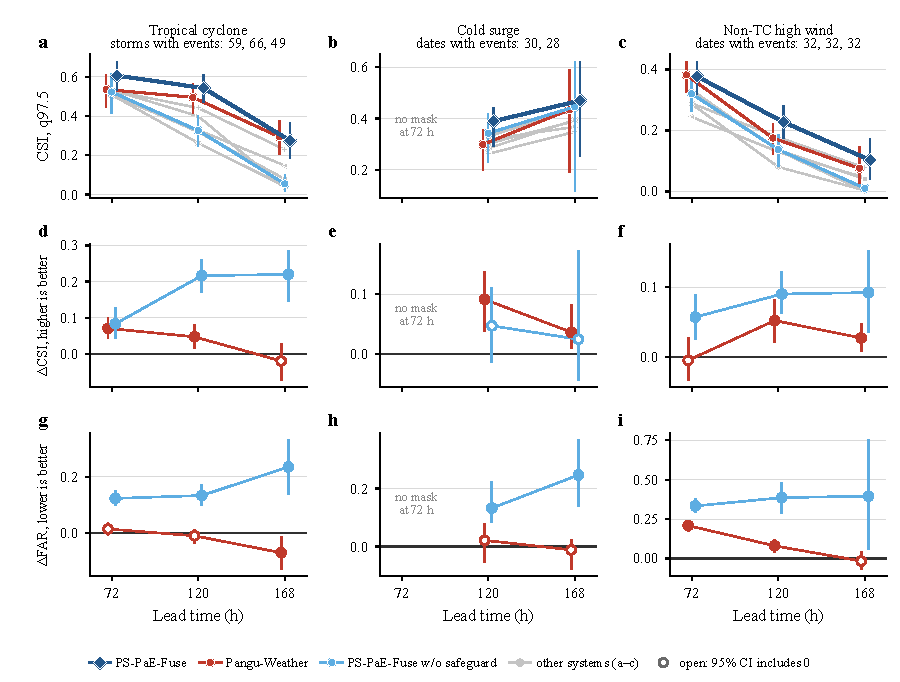
\includegraphics[width=\textwidth]{figS_strata_by_lead_2022.pdf}
\caption{Weather-type scores by lead time on the sealed 2022 sample (frozen models; the lead-resolved accumulators reproduce Table~S4). (a--c) q97.5 CSI with 95\% intervals, other systems in grey; titles give the units with events per lead. (d--f) Paired CSI and (g--i) FAR differences of PS-PaE-Fuse from Pangu-Weather (red) and from the configuration without safeguard (blue), with 95\% intervals from 2\,000 resamples; open symbols: the interval includes zero. Cold-surge masks exist only at 120 and 168 h.}
\label{fig:strata_lead}
\end{figure}


\clearpage
\section{Skill--detection frontier of the objective experiment}

\begin{figure}[h!]
\centering
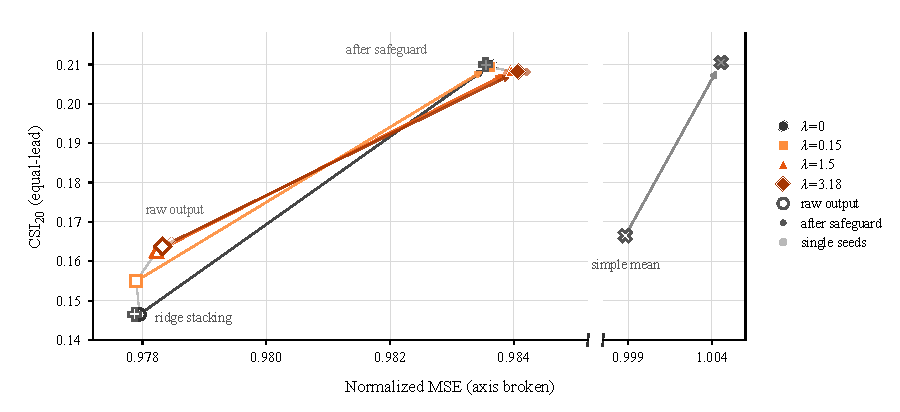
\includegraphics[width=\textwidth]{figS_frontier_2021.pdf}
\caption{Normalized MSE against equal-lead CSI$_{20}$ for the four training objectives of the 2021 objective experiment (three-seed means, small symbols: single seeds), raw (open) and after the common safeguard (filled), with the ridge and simple-mean controls of Table~5 of the main text. The axis is broken because the simple mean lies about 0.02 higher in normalized MSE.}
\label{fig:frontier}
\end{figure}

\end{document}
